\section{Overview}
Boxcom measures the current it sources into a 3.3V output voltage.  It
can be used to estimate the battery life of devices using popular 3V
coin cells, such as the one shown in figure \ref{fig:coincell}.  Boxcom features:
\begin{itemize}
  \item 20mA maximum output current with 100$\mu$A resolution
  \item USB port providing power and virtual COM port connection to PC
  \item Open ASCII command set for data collection
  \item Open-source, cross-platform host software written in Python
    using Tkinter widgets and Matplotlib for plotting.
\end{itemize}

\begin{figure}[ht]
  \begin{center}
    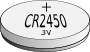
\includegraphics[clip,scale=1]{figs/coincell}
    \caption{Boxcom can be connected in place of 3V coin
      cells to measure a device's current draw.\label{fig:coincell}}
    \end{center}
\end{figure}